\section{Project management}

\begin{definition}[\textit{Project}]
    A project is a set of tasks that must be completed within a defined timeline to achieve specific objectives and deliverables.
\end{definition}
\noindent A project is characterized by its scope, which defines the goals, deliverables, and constraints. 
It involves multiple stakeholders and is executed by a dedicated project team. 
The project's methodology acts as a guiding framework, encompassing processes, methods, and best practices to ensure the successful achievement of project objectives.

The main KPIs or evaluating project success include:
\begin{itemize}
    \item \textit{Revenue}: total income generated by the company from its consulting services before deducting expenses.
    \item \textit{Earning before tax}: measures profitability before accounting for income tax expenses.
    \item \textit{Cost on revenues}: ratio of costs directly associated with generating revenue. 
    \item \textit{Un-allocation}: refers to staff who are not assigned to revenue-generating activities.
\end{itemize}

\subsection{Requirements}
For data teams to deliver effective analytics solutions, collaboration with business stakeholders is essential to understand their needs and desired outcomes. 
A structured requirements-gathering process is critical for determining the appropriate type of analysis and selecting the right solution.
Without clear requirements, data teams cannot accurately define the project scope or develop an effective solution.

\subsection{Project development}
Two primary methodologies dominate project development: Waterfall and Agile. 
Each approach has distinct strengths and limitations, making them suitable for different types of projects.

\subsubsection{Waterfall}
The waterfall model follows a sequential process, where each phase (analysis, design, development, testing, and implementation) progresses linearly.
Once a phase begins, changes to requirements are difficult to incorporate. 
This approach is ideal for projects with well-defined and stable requirements from the outset.

Waterfall methodology is particularly effective for projects requiring strict compliance, comprehensive documentation, and structured processes. 
Key components include project management, the project team, and subject matter experts.

\begin{figure}[H]
    \centering
    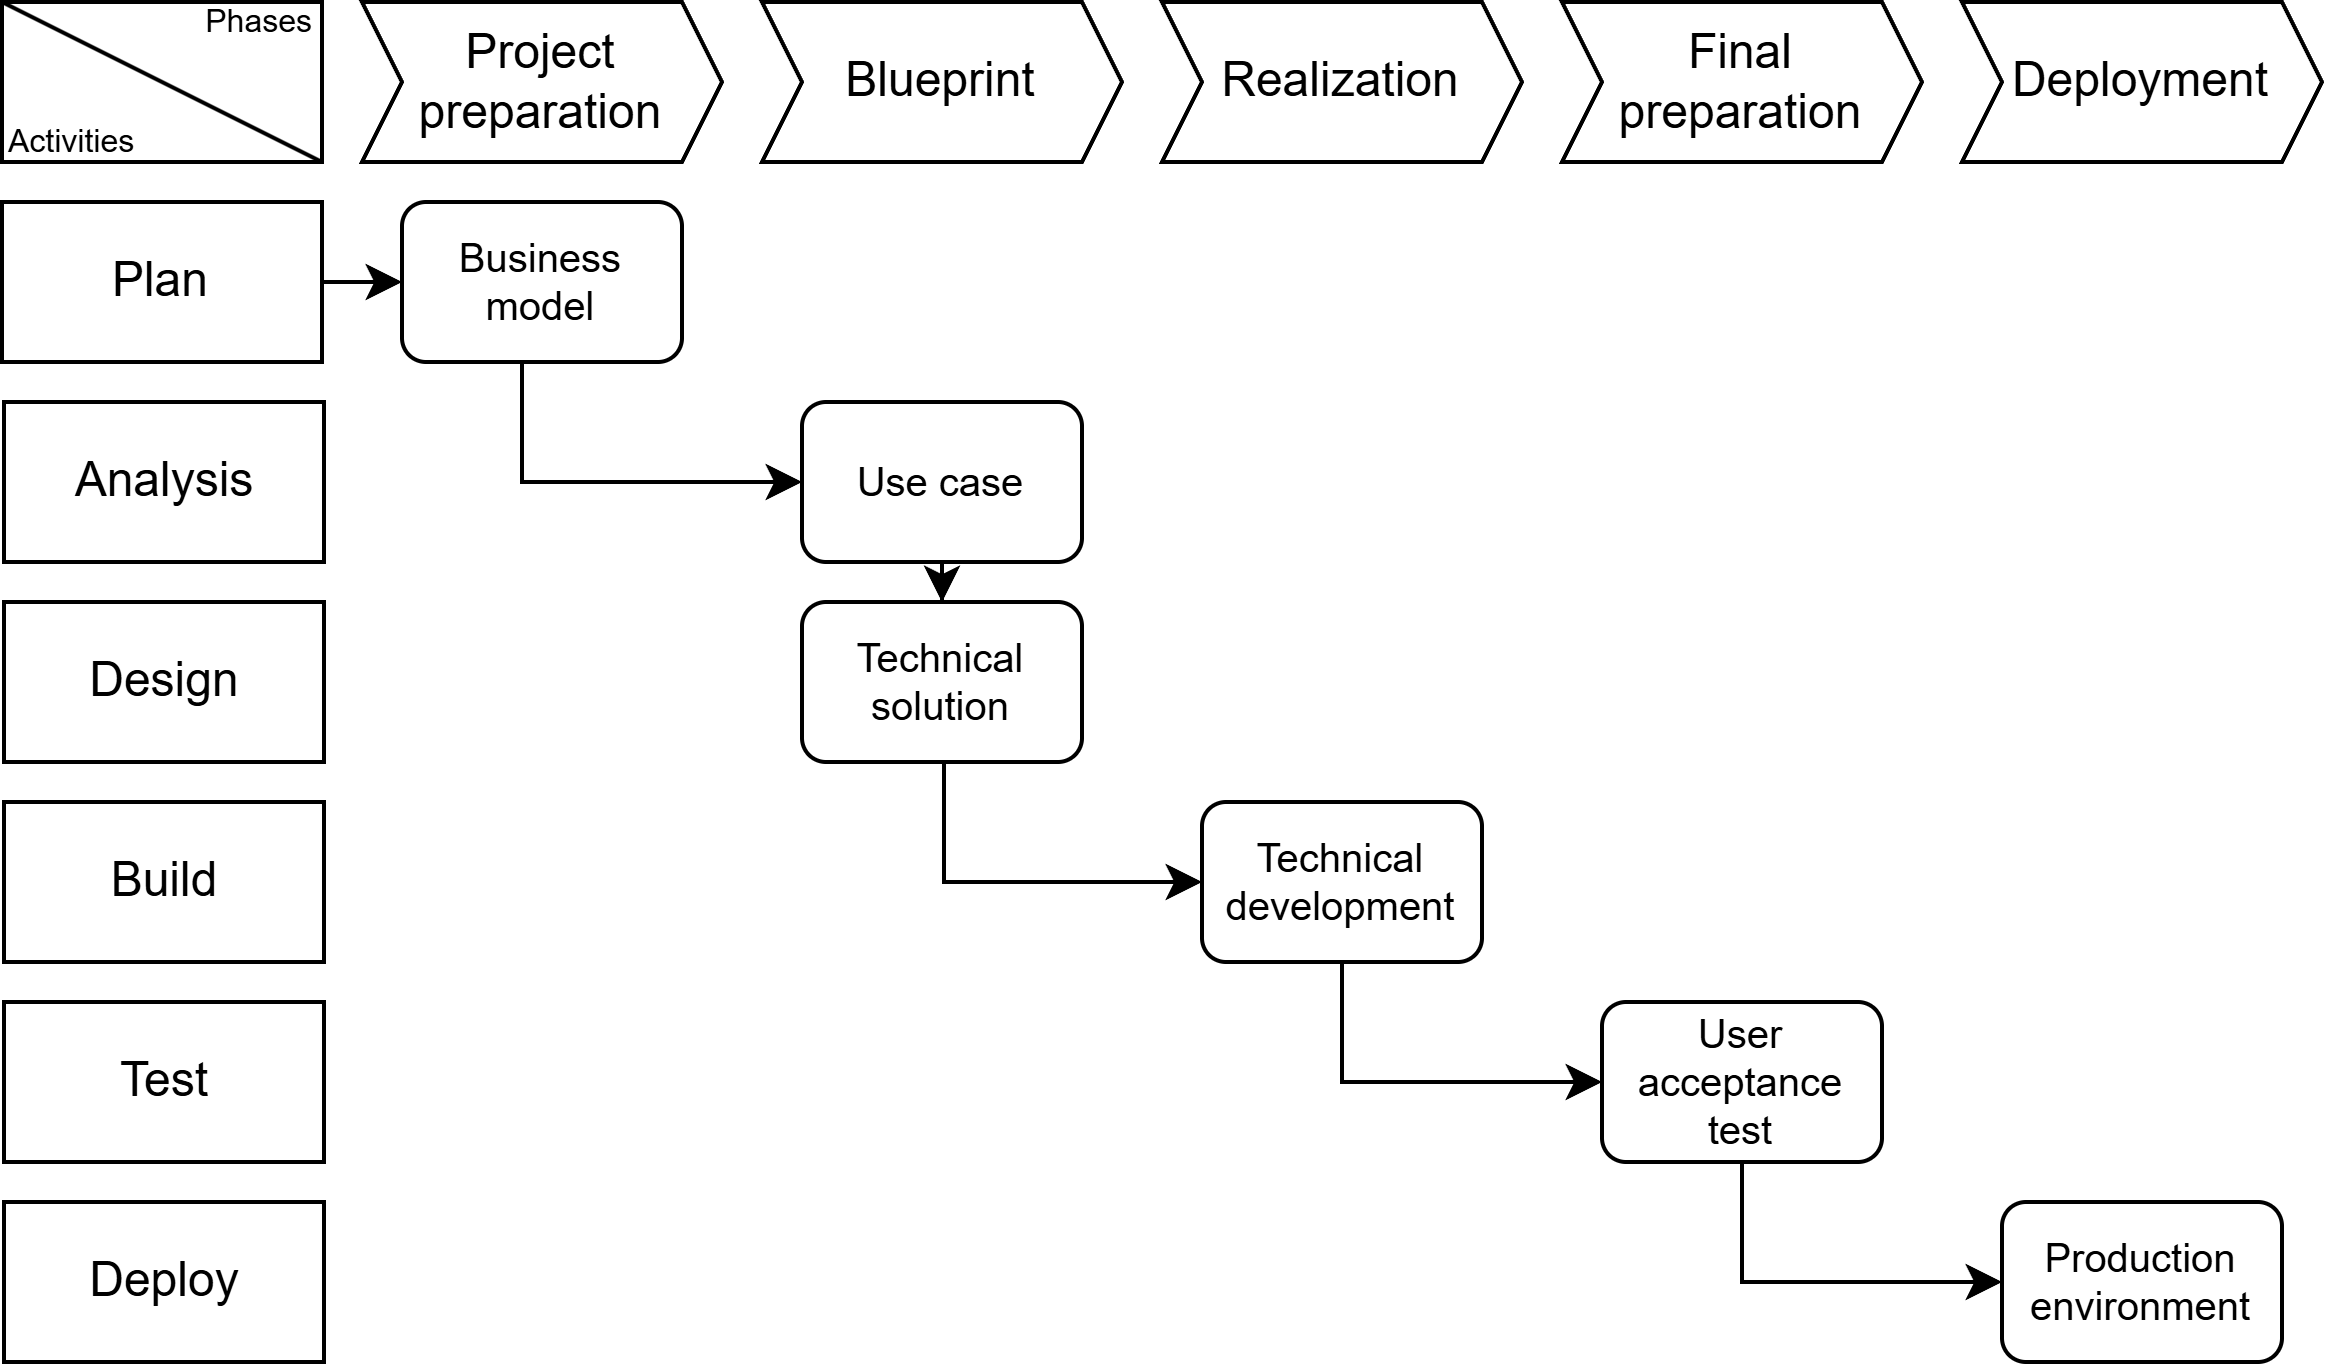
\includegraphics[width=0.75\linewidth]{images/bis8.png}
    \caption{Waterfall project phases}
\end{figure}

\subsubsection{Agile}
Agile adopts an iterative and incremental approach, offering greater flexibility. 
Work is organized into sprints, each delivering a functional product increment. 
Agile emphasizes continuous collaboration with clients and adapts seamlessly to evolving requirements.

Agile is well-suited for projects where requirements may change frequently or when rapid, tangible results are needed.
\noindent Key roles in agile include:
\begin{itemize}
    \item \textit{Product owner}: responsible for defining and communicating the product goal, creating the product backlog, and prioritizing backlog items based on business value.
    \item \textit{Developers}: plan and execute sprints, create the sprint backlog, maintain quality standards, and adjust plans as necessary to meet the sprint goal.
    \item \textit{Scrum master}: acts as a coach for the team, removes obstacles, and ensures focus on delivering high-value increments while adhering to agile principles.
\end{itemize}

\begin{figure}[H]
    \centering
    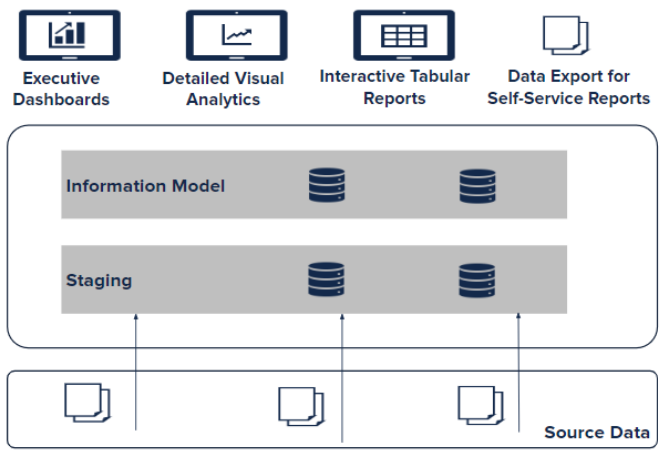
\includegraphics[width=0.5\linewidth]{images/bis9.png}
    \caption{Agile project phases}
\end{figure}

\subsubsection{Hybrid}
A hybrid methodology combines elements of both waterfall and agile, adapting to the unique needs of the project. 
This approach provides flexibility while maintaining structured planning, making it suitable for projects that require a balance of predictability and adaptability.